
% titlepage-demo.tex
\documentclass{beamer}
\usetheme{Boadilla}
\usepackage{multirow}
\usepackage[absolute,overlay]{textpos} 
\newenvironment{reference}[2]{% 
  \begin{textblock*}{\textwidth}(#1,#2) 
      \footnotesize\it\bgroup\color{red!50!black}}{\egroup\end{textblock*}} 

\begin{document}

\begin{frame}{Motivation - Human Way to Detect Event} 
	\begin{center}
		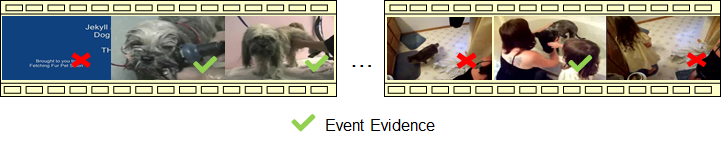
\includegraphics[width=11cm,height=3cm]{images/part4/minimalevidence.png}
	\end{center}
	\begin{itemize}
		\item Human only needs to see some evidences.
		\item Leveraging on positive and negative visual cues selected by humans significantly improves the performance.
	\end{itemize}
 \begin{reference}{4mm}{85mm}
 	Bhattacharya, S., Yu, F. X., Chang, S. F. Minimally needed evidence for complex event recognition in unconstrained videos. In ICMR. ACM, 2014.
 \end{reference}  
\end{frame}

\begin{frame}{Motivation - Not Easy for Computer} 
	\begin{center}
		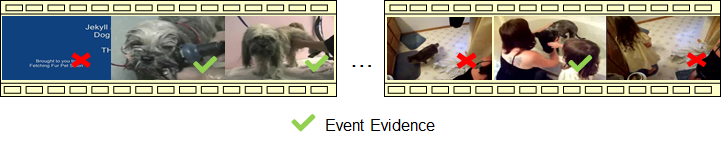
\includegraphics[width=11cm,height=3cm]{images/part4/minimalevidence.png}
	\end{center}
	
	\begin{itemize}
		\item How to detect which segments of the video that have the most contributions? 	
		\item How to leverage these ``\textit{key evidences}'' for event detection?
	\end{itemize}	
	$\rightarrow$ Answering these two questions can help understand why an event is detected.	
\end{frame}

\begin{frame}{Weakly Supervised Learning Problem} 	
	\textbf{\textit{Problem}}: Event labels are only given at video level!
	
	\begin{center}
		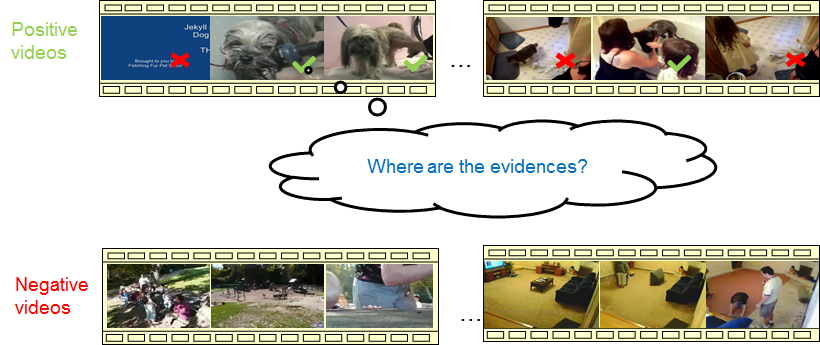
\includegraphics[width=11cm,height=4cm]{images/part4/supervidedlearning.png}
	\end{center}
	
	
	\textbf{Related work} 
	\begin{itemize}	
		\item Latent SVM [Tang-CVPR2012], [Li-ICCV2013]
		\item \textbf{Multiple Instance Learning} [Zhang-ICML2002], [Lai-CVPR2014] 
			\begin{itemize}	
\item Mathematically equivalent to Latent SVM! 
\item MIL can be applied directly to learn labels at segment level: \\
video $\rightarrow$ ``bag'', segment $\rightarrow$ ``instance''.
			\end{itemize}	
	\end{itemize}	

\end{frame}	

\begin{frame}{Multiple Instance Learning - miSVM} 	
	Two key assumptions of MIL:
	\begin{itemize}	
		\item A positive bag has \textbf{at least} one positive instance.
		\item The instances in a negative bag are \textbf{all} negatives.
	\end{itemize}	
	\begin{center}
		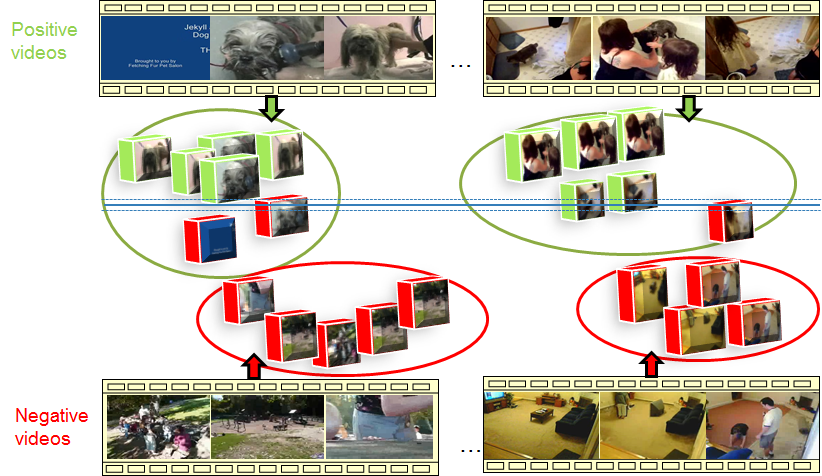
\includegraphics[width=11cm,height=6cm]{images/part4/miSVM.png}
		\\
		\scriptsize{miSVM: instance-based classifier}
	\end{center}
	
\end{frame}	

\begin{frame}{Multiple Instance Learning - MISVM} 	

	\begin{center}
		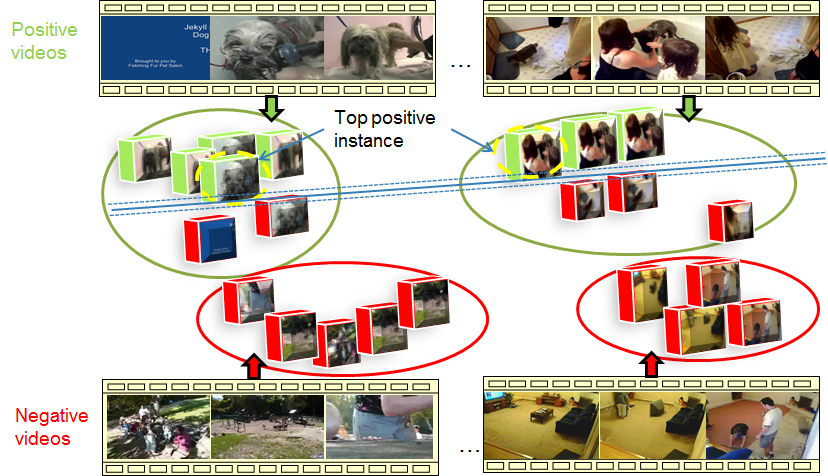
\includegraphics[width=11cm,height=6cm]{images/part4/MI-SVM.png}
		\\
		\scriptsize{MISVM: bag-based classifier}
	\end{center}
\textbf{Limitations}: MIL assumptions may not be valid for videos, esp. \textbf{complex} videos.
\end{frame}	

\begin{frame}{Proportional SVM [Lai-CVPR2014]} 	
	Two new assumptions of p-SVM:
	\begin{itemize}	
		\item Positive videos should have \textbf{high proportion} of positive instances.
		\item Negative videos could have \textbf{some} positive instances.
	\end{itemize}	
	
	\begin{center}
		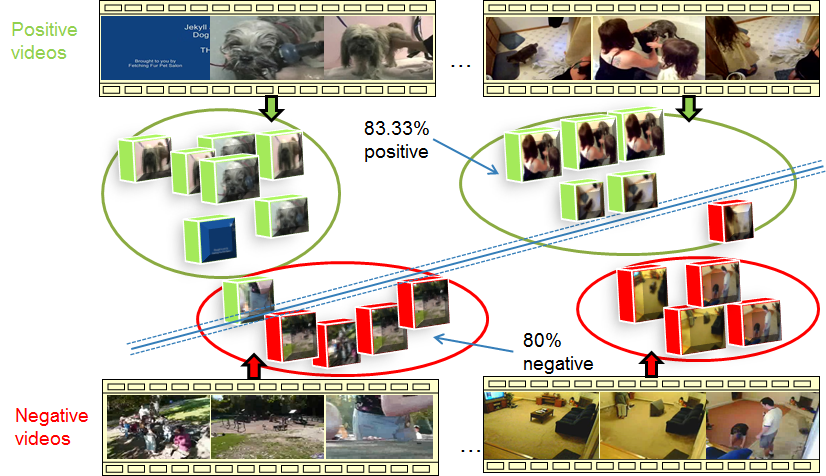
\includegraphics[width=11cm,height=6cm]{images/part4/pSVM.png}
	\end{center}
	
\end{frame}	

\begin{frame}{Our Proposed Method} 	
	
\begin{itemize}	
	\item \textbf{Limitation} of previous work: weakly supervised learning problem
	\begin{itemize}	
		\item Instance labels are solely classified based on its represented feature in a large margin framework.
		\item The importance of each instance is not considered.
	\end{itemize}	
	
	\item What if we know information about the instance labels?
		\begin{itemize}	
			\item E.g., the relatedness of each instance to the event of interest.
		\end{itemize}	
		\begin{center}
			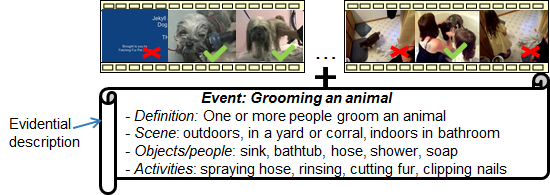
\includegraphics[width=9cm,height=4cm]{images/part4/eventkit.png}
		\end{center}
	\item \textbf{Our proposed method}: A ``stronger'' supervised learning problem
		\begin{itemize}	
			\item Event-driven Multiple Instance Learning (EDMIL) to utilize the \textit{evidential description} for event detection.
		\end{itemize}	

\end{itemize}	
	
\end{frame}	

\begin{frame}{Instance-Event Similarity} 	
	\begin{itemize}	
		\item Adopt a \textbf{concept expansion} strategy [Wang ICMR2014]
				\begin{itemize}	
					\item Apply at instance level
				\end{itemize}	
	\item consists of 4 steps:
	
		\begin{itemize}
			\item Concept detection.
			\item Event representation (text-based).
			\item Concept-event similarity.
			\item Instance-event similarity.
		\end{itemize}
		
	\end{itemize}		
	\begin{center}
		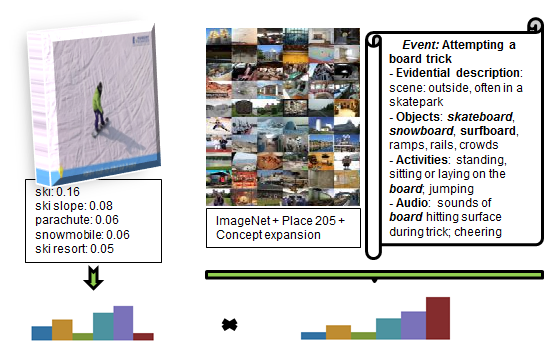
\includegraphics[width=9cm,height=4.7cm]{images/part4/similarity.png}
	\end{center}

\end{frame}	

\begin{frame}{Instance-Event Similarity (cont'd)} 	

% Please add the following required packages to your document preamble:
% \usepackage{booktabs}
\begin{table}[h]
	\scriptsize
		\caption{Top five concepts discovered by our system for the first 10 events in the MED 2012 dataset.}
		\renewcommand{\arraystretch}{0.8}
	\begin{tabular}{@{}ll@{}}
		\toprule
		\multicolumn{1}{c}{\textbf{Event name}}                & \multicolumn{1}{c}{\textbf{Top five importance concepts discovered by our system}}                                                  \\ \midrule
		\multicolumn{1}{|l|}{Attempting a board trick}         & \multicolumn{1}{l|}{Ski, slide rule, ski resort, ski mask, ice skating rink}                                                        \\ \midrule
		\multicolumn{1}{|l|}{Feeding an animal}                & \multicolumn{1}{l|}{Meat loaf, white shark, food court, pop bottle, cleaver}                                                        \\ \midrule
		\multicolumn{1}{|l|}{Landing a fish}                   & \multicolumn{1}{l|}{Anemone fish, pole, raft, sturgeon, boat deck}                                                                  \\ \midrule
		\multicolumn{1}{|l|}{Wedding ceremony}                 & \multicolumn{1}{l|}{Groom, bridegroom, banquet hall, gown, altar}                                                                   \\ \midrule
		\multicolumn{1}{|l|}{Working on a woodworking project} & \multicolumn{1}{l|}{\begin{tabular}[c]{@{}l@{}}Jigsaw puzzle, bamboo forest, carpenter's kit, thatch,\\  wooden spoon\end{tabular}} \\ \midrule
		\multicolumn{1}{|l|}{Birthday party}                   & \multicolumn{1}{l|}{Table lamp, lampshade, torch, candle, custard apple}                                                            \\ \midrule
		\multicolumn{1}{|l|}{Changing a vehicle tire}          & \multicolumn{1}{l|}{\begin{tabular}[c]{@{}l@{}}Recreational vehicle, car wheel, amphibian, scooter,\\  sports car\end{tabular}}     \\ \midrule
		\multicolumn{1}{|l|}{Flash mob gathering}              & \multicolumn{1}{l|}{Monitor, chime, bell, whistle, ballroom}                                                                        \\ \midrule
		\multicolumn{1}{|l|}{Getting a vehicle unstuck}        & \multicolumn{1}{l|}{\begin{tabular}[c]{@{}l@{}}Recreational vehicle, amphibian, tank, car wheel,\\  motor scooter\end{tabular}}     \\ \midrule
		\multicolumn{1}{|l|}{Grooming an animal}               & \multicolumn{1}{l|}{Nail, bathtub, shower, fur coat, washbashin}                                                                    \\ \bottomrule
	\end{tabular}
\end{table}
	
\end{frame}	

\begin{frame}{Event-driven Multiple Instance Learning} 	
	
	\begin{itemize}	
		\item $V$: number of training videos
		\item $I_{v}$: number of instances in video $v$
		\item $S_{iv}^{e}$: similarity between instance $iv$ and event $e$ 
		\item R: number of level of relatedness from an instance to an event
	\end{itemize}
We define two predict functions for positive and negative instances at level $r$ as follows. \\
	\begin{center}
$
P_{pos}(S_{iv}^{e},r) = 
\begin{cases}
1,& \text{if } Rank(S_{iv}^{e}) \leq r \\
-1,              & \text{otherwise}
\end{cases}
$

$
P_{neg}(S_{iv}^{e},r) = 
\begin{cases}
-1,& \text{if } Rank(S_{iv}^{e}) \leq r \\
1,              & \text{otherwise}
\end{cases}
$
\end{center}

$Rank(.)$ is the function to quantize a similarity into a related level.
\textbf{Intuition}: we can select the top positive and negative instances at each level of relatedness $r$.
\end{frame}	



\begin{frame}{Event-driven Multiple Instance Learning} 	
		\begin{itemize}	
			\item Objective function
		\end{itemize}	
	\begin{center}
		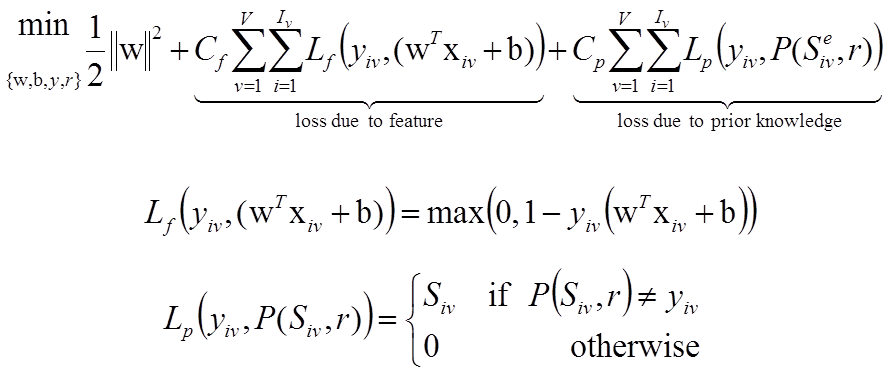
\includegraphics[width=10cm,height=4.5cm]{images/part4/formalization.png}
		\\
		$C_{f}$, $C_{p}$: cost parameters to control the influence of each loss function.\\
				
	\end{center}
\begin{itemize}	
	\item Mixed-integer programming problem $\rightarrow$ \textbf{non-convex optimization}!
\end{itemize}	
	
\end{frame}	

\begin{frame}{Optimization Procedure} 	

		\textbf{Alternating optimization strategy} to search for a suboptimal solution:

\begin{enumerate}
	\item Fix instance labels $y_{iv}$ and solve for \textbf{w} and \textit{b} $\rightarrow$ classic SVM problem:
	
		\begin{center}
	\small{$\min\limits_{\textbf{w},b}$ $\frac{1}{2} \left \| \textbf{w} \right \|^{2} + C_{f} \sum_{v=1}^{V}\sum_{i=1}^{I_{v}}L_{f}\left ( y_{iv}, \textbf{w}^{T}\textbf{x}_{iv}+b \right )$}
		\end{center}
	
	\item Fix \textbf{w} and \textit{b}, solve for $r$ and update $y_{iv}$:
	
		\begin{center}
	\small{$\min\limits_{y,r} C_{f} \sum_{v=1}^{V}\sum_{i=1}^{I_{v}}L_{f}\left ( y_{iv}, \textbf{w}^{T}\textbf{x}_{iv}+b \right )
	+ C_{p} \sum_{v=1}^{V}\sum_{i=1}^{I_{v}}L_{p}\left ( y_{iv}, P(S_{iv}^{e},r) \right )$}
		\end{center}
		
		Solved by using a \textbf{greedy strategy}: 
		\begin{itemize}
			\item Iterate through all level of relatedness to search for the optimal $r$.
			\item Update instance labels $y_{iv}$ using the proposed predict functions.
		\end{itemize}
		\textbf{Intuition}: the most positive and negative instances will be selected first $\rightarrow$ higher possibility to correct mismatched labels.
\end{enumerate}
	
	
\end{frame}	

\begin{frame}{Experimental Setup} 	
	\begin{itemize}
		\item Dataset

\begin{table}[h]
	\tiny
	\begin{tabular}{@{}|l|c|c|c|c|c|@{}}
		\toprule
		\multicolumn{1}{|c|}{Dataset} & No. Event & No. Train Videos & No. Test Videos & Total Videos & Total Hours \\ \midrule
		\light{MED2010} & \light{3} & \light{1,744} & \light{1,724} & \light{3,468} & \light{110 hours} \\ \midrule
		MED2011 & 10 & 1,331 & 31,822 & 33,153 & 1,100 hours \\ \midrule
		MED2012 & 25 & 3,878 & 1,938 & 5,816 & 250 hours \\ \bottomrule
	\end{tabular}
\end{table}

\item Segment length: 8 seconds [Vahdat ICCV2013]
\item Feature: Improved Dense Trajectories, MBH descriptor [Wang ICCV2013] 
\item Feature encoding: Bag-of-words model, 4000 codewords.
\item Learning: EDMIL (with linear SVM).
\item Testing: Video-level score is obtained by averaging over all instance scores.
	\end{itemize}
		
\end{frame}	


\begin{frame}{Optimal Number of Related Levels} 	
	Select R in the range from 1 to 10 and report the best result.
		\begin{center}
			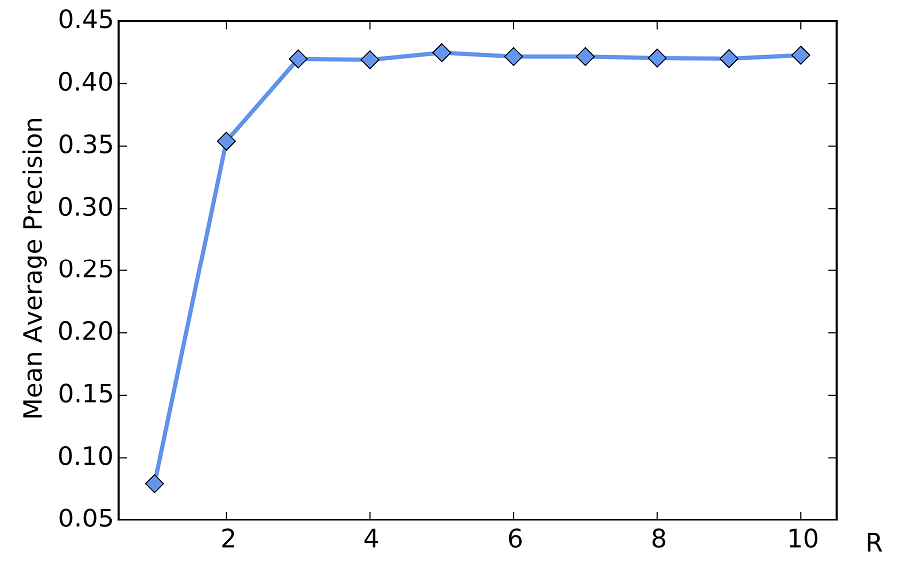
\includegraphics[width=7cm,height=4.5cm]{images/part4/optimalR.png}
		\end{center}

	\begin{itemize}
		\item Small	values of R tend to get low performances $\rightarrow$ the prediction of prior knowledge is not always good, and learning jointly with instance features is necessary.
		\item The performance becomes saturated when R $>$ 5 $\rightarrow$ we fix the value of R to 5 for further experiments.
	\end{itemize}
		
\end{frame}	

\begin{frame}{Results on MED2012} 	
	\begin{center}
		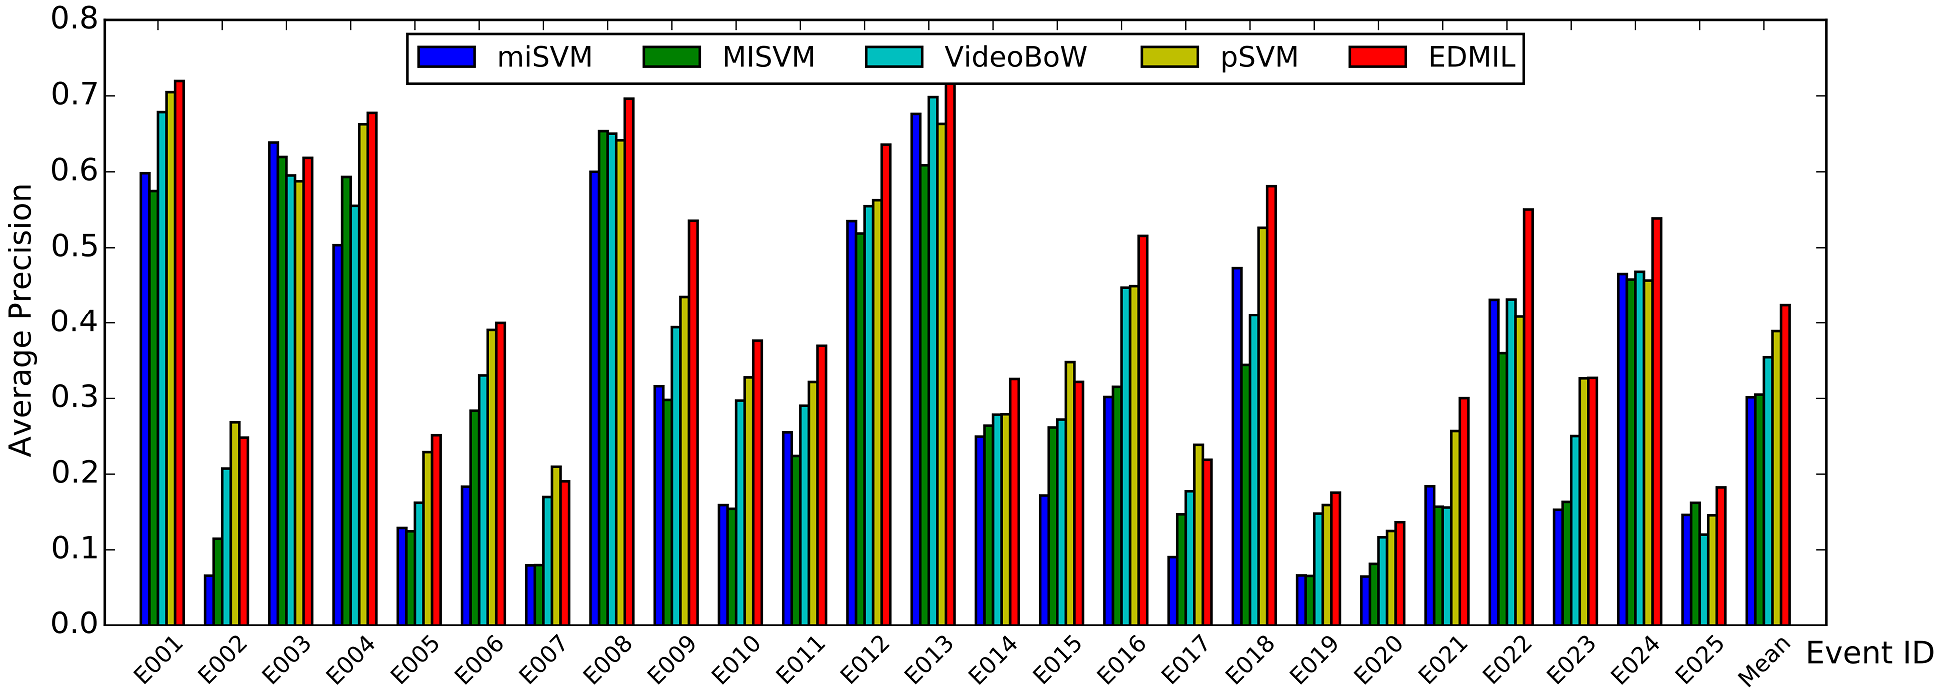
\includegraphics[width=12cm,height=5cm]{images/part4/med12.png}
		\\
		\tiny{The mean APs are 0.3015 (miSVM), 0.3051 (MISVM), 0.3544 (VideoBOW), 0.3890 (pSVM) and \textbf{0.4246} (\textbf{Ours}).}
	\end{center}
	
	\begin{itemize}
		\item Our method significantly outperforms other baselines.
		\item For the best baseline (pSVM), our method relatively outperforms by 9\%. 	
	\end{itemize}
	
\end{frame}	

\begin{frame}{Results on MED2011} 	
	\begin{center}
		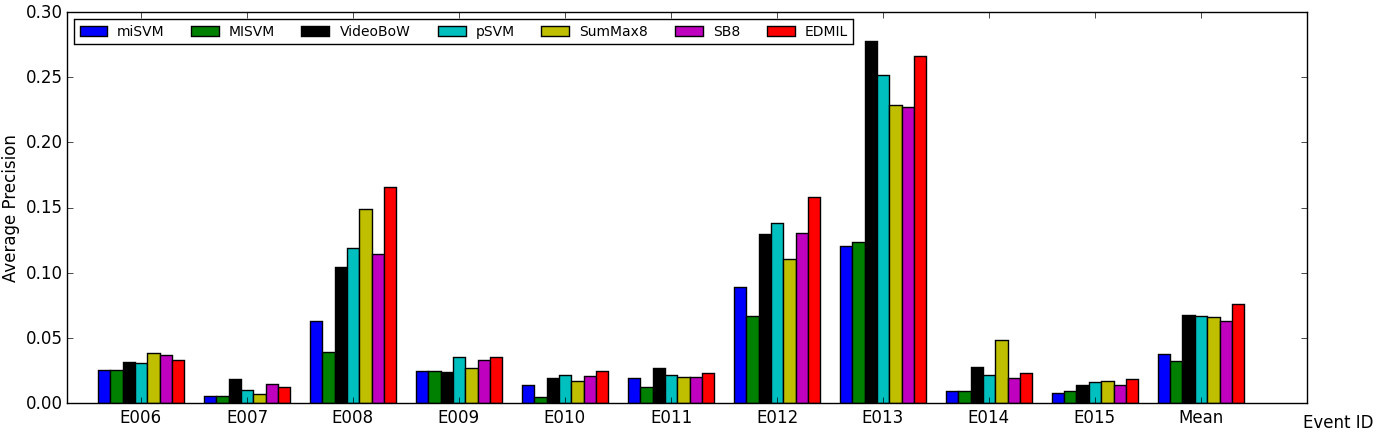
\includegraphics[width=12cm,height=4.5cm]{images/part4/sum_med11_2.png}
		\\
		\tiny{MAP: 0.0378 (miSVM), 0.0322 (MISVM), 0.0674 (VideoBOW), 0.0666 (pSVM), 0.0663 (SM8), 0.0630 (SB8), \textbf{0.0761} (\textbf{Ours}).}
	\end{center}
	
	\begin{itemize}
		\item Our method still performs well (\textbf{13\%} improvement over the VideoBOW baseline) while pSVM does not.
		%\item miSVM performs better than MISVM $\rightarrow$ instance-based learning is more effective.
	\end{itemize}
(At the testing step: Video-level score is obtained by \textbf{averaging} its instance scores.)	
\end{frame}	

\begin{frame}{Results on MED2011} 	
At the testing step: Video-level score is obtained by choosing the \textbf{max} instance score.	
	\begin{center}
		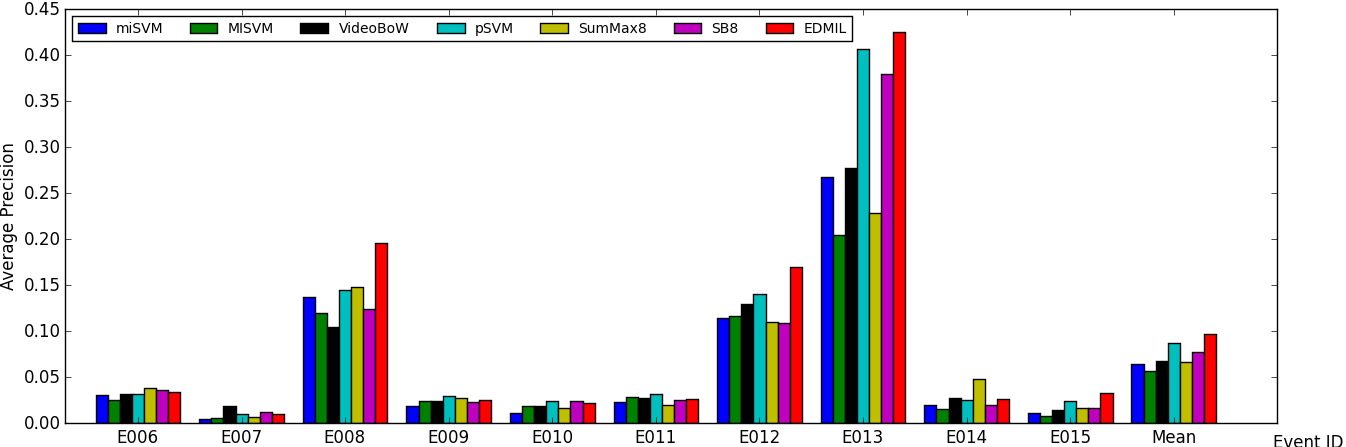
\includegraphics[width=12cm,height=4.5cm]{images/part4/max_med11_2.png}
		\\
		\tiny{MAP: 0.0640 (miSVM), 0.0564 (MISVM), 0.0674 (VideoBOW), 0.0870 (pSVM), 0.0663 (SM8), 0.0770 (SB8), \textbf{0.0968} (\textbf{Ours}).}
	\end{center}
	
	\begin{itemize}
		\item All methods perform better with this strategy.
		\item Our method relatively outperforms VideoBOW by \textbf{44}\%, and pSVM by \textbf{11}\%. 	
	\end{itemize}
	
\end{frame}	

\begin{frame}{How to Leverage ``\textit{Key Evidences}'' for Event Detection?} 	
	$\rightarrow$ At the testing step, video-level score should be obtained by choosing the \textbf{max} instance score.	
	\begin{center}
		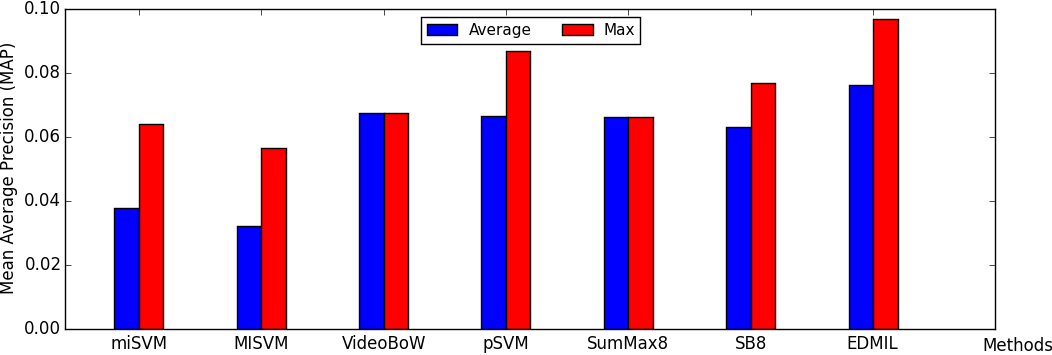
\includegraphics[width=12cm,height=4.5cm]{images/part4/summaxgain.png}
		\\
		Performance gain when choosing the video score as its \textbf{max} instance scores instead of its \textbf{average} instance scores.
	\end{center}
	
\end{frame}	

%\begin{frame}{Top Positive Instances for Event ``Birthday Party''} 	
%
%	\begin{center}
%		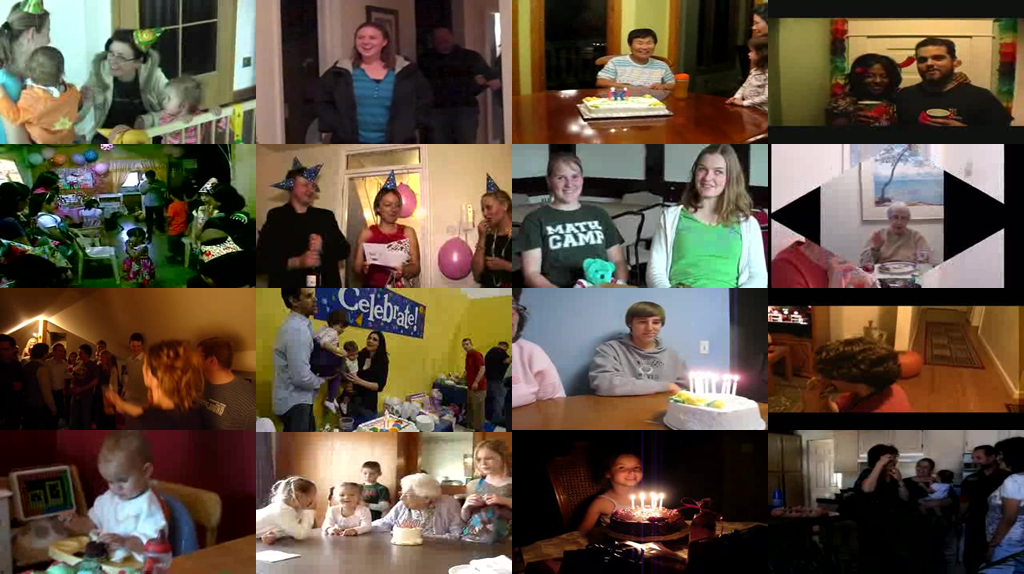
\includegraphics[width=12cm,height=7cm]{images/part4/birthdayparty.png}
%	\end{center}
%	
%\end{frame}	
%
%\begin{frame}{Top Negative Instances for Event ``Birthday party''} 	
%	
%	\begin{center}
%		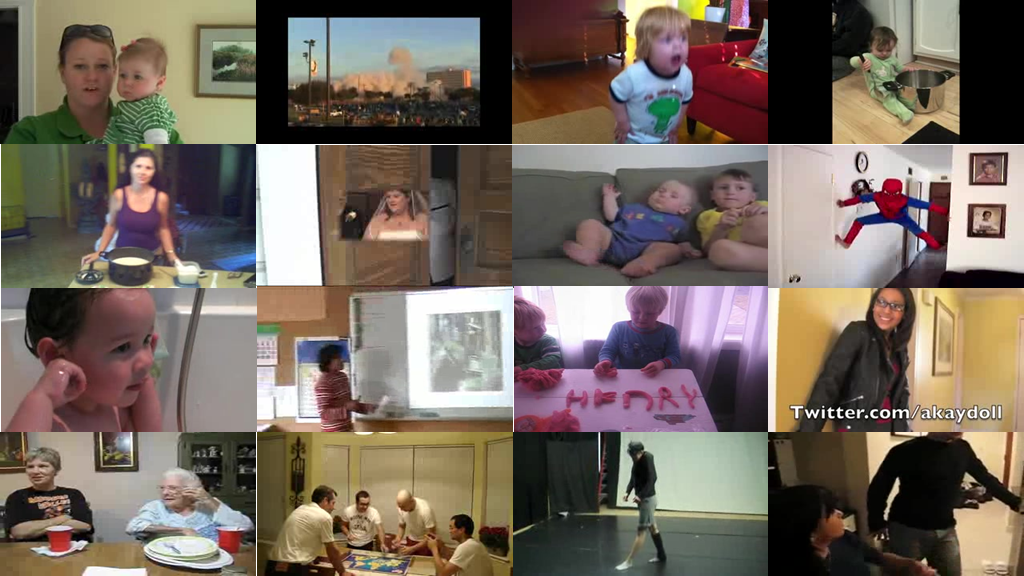
\includegraphics[width=12cm,height=7cm]{images/part4/birthdayparty_neg.png}
%	\end{center}
%	
%\end{frame}	
%
%\begin{frame}{Top Positive Instances for Event ``Flash mob gathering''} 	
%	
%	\begin{center}
%		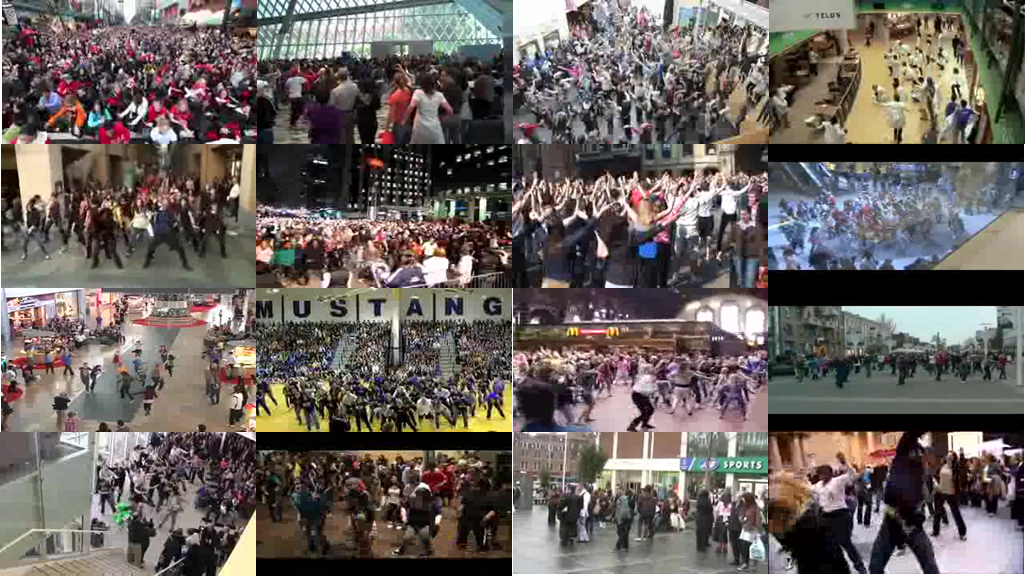
\includegraphics[width=12cm,height=7cm]{images/part4/flashmob.png}
%	\end{center}
%	
%\end{frame}	
%
%\begin{frame}{Top Negative Instances for Event ``Flash mob gathering''} 	
%	
%	\begin{center}
%		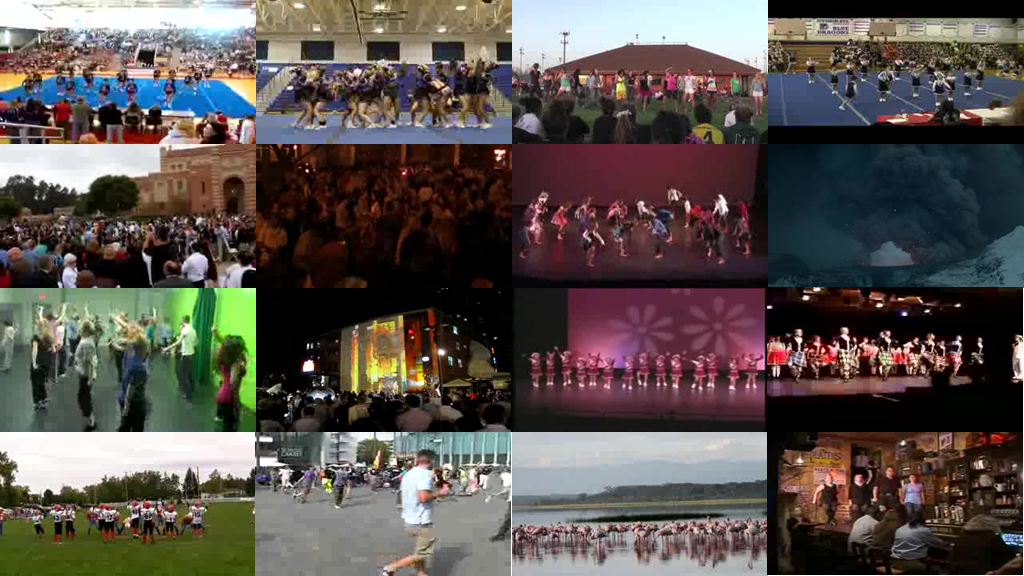
\includegraphics[width=12cm,height=7cm]{images/part4/flashmob_neg.png}
%	\end{center}
	
%\end{frame}	

%\begin{frame}{Top Positive Instances for Event ``Parade''} 	
	
%	\begin{center}
%		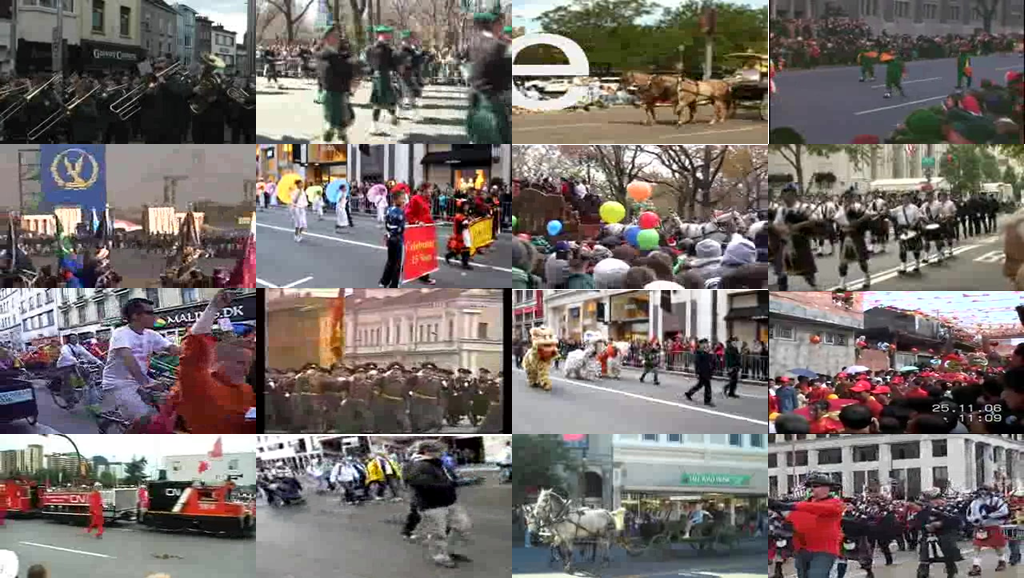
\includegraphics[width=12cm,height=7cm]{images/part4/parade.png}
%	\end{center}
	
%\end{frame}	

%\begin{frame}{Top Negative Instances for Event ``Parade''} 	
	
%	\begin{center}
%		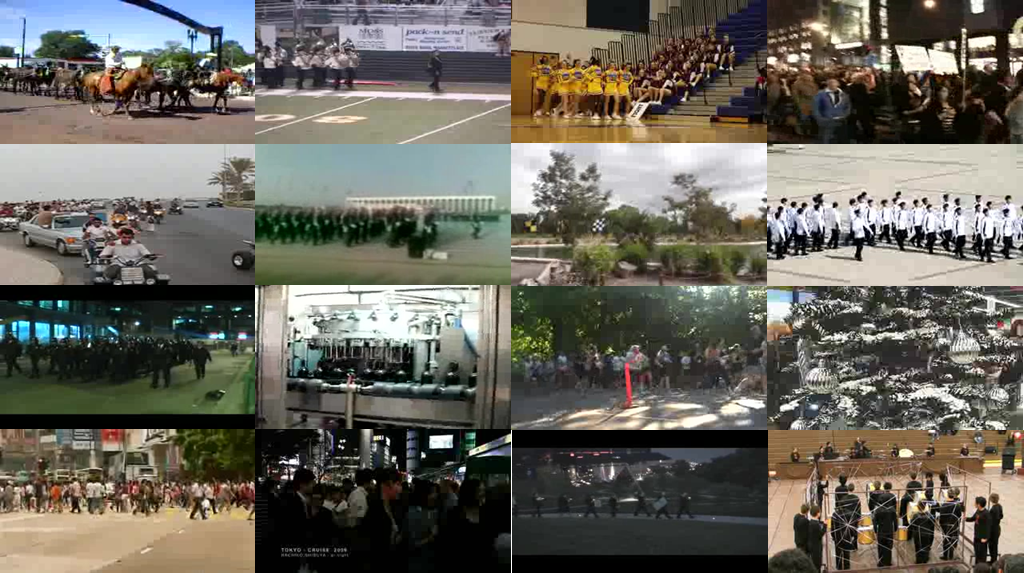
\includegraphics[width=12cm,height=7cm]{images/part4/parade_neg.png}
%	\end{center}
	
%\end{frame}	

\begin{frame}{Top Positive Instances for Event ``Parkour''} 	
\small{\textit{Parkour}: A person travels by foot from one point to another while performing various gymnastic maneuvers.}	
	\begin{center}
		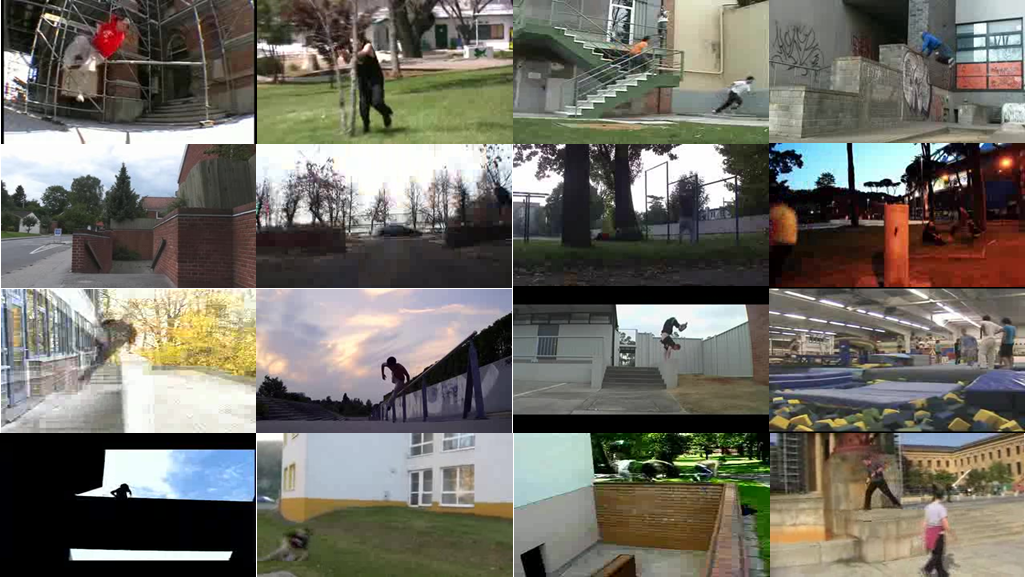
\includegraphics[width=12cm,height=7cm]{images/part4/parkour.png}
	\end{center}
	
\end{frame}	

\begin{frame}{Top Negative Instances for Event ``Parkour''} 	
\small{\textit{Parkour}: A person travels by foot from one point to another while performing various gymnastic maneuvers.}	
	\begin{center}
		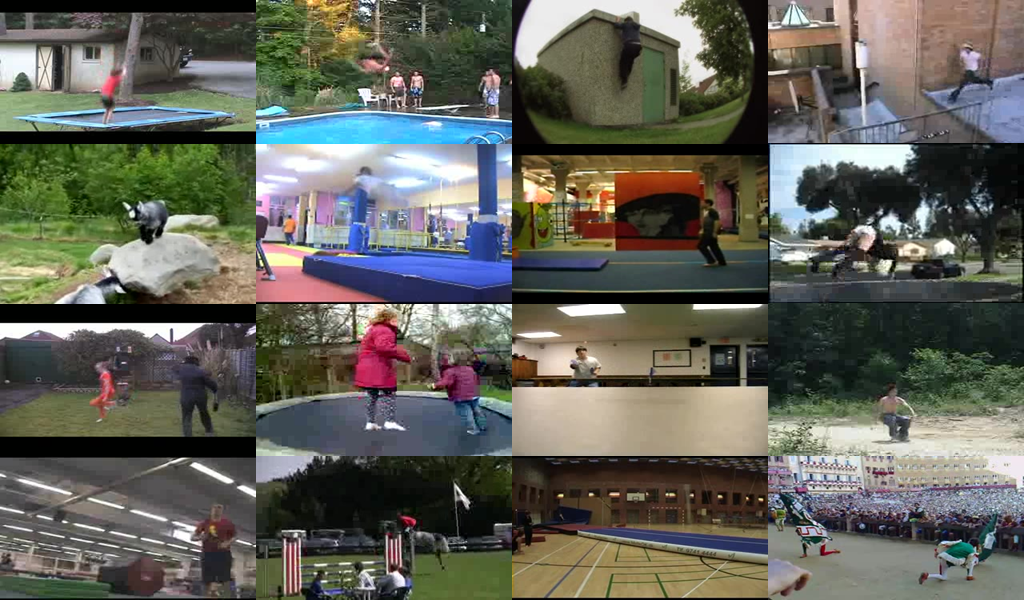
\includegraphics[width=12cm,height=7cm]{images/part4/parkour_neg.png}
	\end{center}
	
\end{frame}	



\begin{frame}[t]{Conclusions}
	
	\begin{enumerate}
		\item \light{Segment-based Representation (SB)}
		\item \light{Sum-Max Video Aggregation (SM)}
		\item \textbf{Event-driven Multiple Instance \\
		Learning (EDMIL)}
		\begin{itemize}
			\item A method to leverage the event\\
			description to learn key evidences \\
			for complex event detection.
		\end{itemize}
	\end{enumerate}
	
	\begin{tikzpicture}[remember picture,overlay]  
	\node [xshift=-3cm,yshift=-4.5cm] at (current page.north east)
	{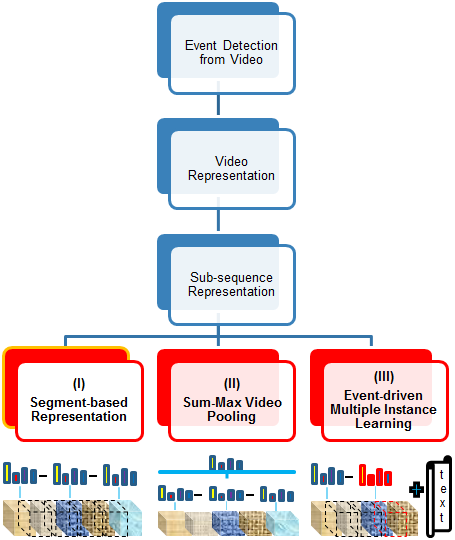
\includegraphics[width=5cm,height=7.5cm]{images/part1/contribution2.png}};
	\end{tikzpicture}
	
\end{frame}


\end{document}